\section{Drawing}
\tkzname{\tkznameofpack} can draw 5 types of objects : point, line or line segment, circle, arc and sector.

%<---------------------------------------------------------------------------->
%    POINT(S)
%<---------------------------------------------------------------------------->
\subsection{Draw a point or some points}
There are two possibilities : \tkzcname{tkzDrawPoint} for a single point or \tkzcname{tkzDrawPoints} for one or more points.

\subsubsection{Drawing points \tkzcname{tkzDrawPoint}} \hypertarget{tdrp}{}

\begin{NewMacroBox}{tkzDrawPoint}{\oarg{local options}\parg{name}}%
\begin{tabular}{lll}%
arguments &  default & definition                 \\
\midrule
\TAline{name of point} {no default}  {Only one point name is accepted}
\bottomrule
\end{tabular}

\medskip
The argument is required. The disc takes the color of the circle, but  lighter. It is possible to change everything. The point is a node and therefore it is invariant if the drawing is modified by scaling.

\medskip
\begin{tabular}{lll}%
\toprule
options             & default & definition \\
\midrule
\TOline{\TIKZ\ options}{}{all \TIKZ\ options are valid.}
\TOline{shape}  {circle}{Possible \tkzname{cross} or \tkzname{cross out}}
\TOline{size}   {6}{$6 \times$ \tkzcname{pgflinewidth}}
\TOline{color}  {black}{the default color can be changed }
\bottomrule
\end{tabular}

\medskip
{We can create other forms such as \tkzname{cross}}
\end{NewMacroBox}

By default, \tkzname{point style } is defined  like this :

\begin{tkzltxexample}[]
  \tikzset{point style/.style = {%
           draw         = black,
           inner sep    = 0pt,
           shape        = circle,
           minimum size = 3 pt,
           fill         = black
                               }
        } 
\end{tkzltxexample}

\subsubsection{Example of point drawings}
Note that \tkzname{scale} does not affect the shape of the dots. Which is normal.  Most of the time, we are satisfied with a single point shape that we can define from the beginning, either with a macro or by modifying a configuration file.

\begin{tkzexample}[latex=5cm,small]
  \begin{tikzpicture}[scale=.5]
   \tkzDefPoint(1,3){A}
   \tkzDefPoint(4,1){B}
   \tkzDefPoint(0,0){O}
   \tkzDrawPoint[color=red](A)
   \tkzDrawPoint[fill=blue!20,draw=blue](B)
   \tkzDrawPoint[shape=cross,size=8pt,color=teal](O)
  \end{tikzpicture}
\end{tkzexample}

It is possible to draw several points at once but this macro is a little slower than the previous one. Moreover, we have to make do with the same options for all the points.
\newpage
\hypertarget{tdrps}{}
\begin{NewMacroBox}{tkzDrawPoints}{\oarg{local options}\parg{liste}}%
\begin{tabular}{lll}%
arguments &  default  & definition \\
\midrule
\TAline{points list}{no default}{example \tkzcname{tkzDrawPoints(A,B,C)}}
\bottomrule
\end{tabular}

\medskip
\begin{tabular}{lll}%
options             & default & definition \\
\midrule
\TOline{shape}  {circle}{Possible \tkzname{cross} or \tkzname{cross out}}
\TOline{size}  {6}{$6 \times$ \tkzcname{pgflinewidth}}
\TOline{color}  {black}{the default color can be changed }
\bottomrule
\end{tabular}

\medskip
\tkzHandBomb\ Beware of the final "s", an oversight leads to cascading errors if you try to draw multiple points. The options are the same as for the previous macro.
\end{NewMacroBox}

\subsubsection{Example}

\begin{tkzexample}[latex=7cm,small]
\begin{tikzpicture}
\tkzDefPoints{1/3/A,4/1/B,0/0/C}
\tkzDrawPoints[size=3,color=red,fill=red!50](A,B,C)
\end{tikzpicture}
\end{tkzexample}
%<---------------------------------------------------------------------------->
%    LINE(S)
%<---------------------------------------------------------------------------->
\section{Drawing the lines}
The following macros are simply used to draw, name lines.
\subsection{Draw a straight line}
To draw a normal straight line, just give a couple of points. You can  use the \tkzname{add} option to extend the line (This option is due to \tkzimp{Mark Wibrow}, see the code below). 

The style of a line is by default :

\begin{tkzltxexample}[]
  \tikzset{line style/.style = {%
    line width = 0.6pt,
    color      = black,
    style      = solid,
    add        = {.2} and  {.2}%
   }}
\end{tkzltxexample}
with
   
\begin{tkzltxexample}[]
  \tikzset{%
    add/.style args={#1 and #2}{
        to path={%
 ($(\tikztostart)!-#1!(\tikztotarget)$)--($(\tikztotarget)!-#2!(\tikztostart)$)%
  \tikztonodes}}}
\end{tkzltxexample}

You can modify this style with \tkzcname{tkzSetUpLine} see \ref{tkzsetupline}

\newpage
\begin{NewMacroBox}{tkzDrawLine}{\oarg{local options}\parg{pt1,pt2} }%
The arguments are a list of two points or three points. It would be possible, as for a half line, to create a style with \tkzcname{add}.

\begin{tabular}{lll}%
\toprule
options             & default & definition                         \\ 
\midrule
\TOline{\TIKZ\ options}{}{all \TIKZ\ options are valid.}
\TOline{add}{0.2 and 0.2}{add = $kl$ and $kr$, \dots}
\TOline{\dots}{\dots}{allows the segment to be extended to the left and right. }
\bottomrule
\end{tabular}

\tkzname{add} defines the length of the line passing through the points pt1 and pt2. Both numbers are percentages. The styles of \TIKZ\ are accessible for plots.
\end{NewMacroBox}

\subsubsection{Examples  with \tkzname{add}}
\begin{tkzexample}[latex=5cm,small]
\begin{tikzpicture}
 \tkzInit[xmin=-2,xmax=3,ymin=-2.25,ymax=2.25]
 \tkzClip[space=.25]
 \tkzDefPoint(0,0){A} \tkzDefPoint(2,0.5){B}
 \tkzDefPoint(0,-1){C}\tkzDefPoint(2,-0.5){D} 
 \tkzDefPoint(0,1){E} \tkzDefPoint(2,1.5){F} 
 \tkzDefPoint(0,-2){G} \tkzDefPoint(2,-1.5){H}
 \tkzDrawLine(A,B)    \tkzDrawLine[add = 0 and .5](C,D) 
 \tkzDrawLine[add = 1 and 0](E,F)
 \tkzDrawLine[add = 0 and 0](G,H) 
 \tkzDrawPoints(A,B,C,D,E,F,G,H)    
 \tkzLabelPoints(A,B,C,D,E,F,G,H)  
\end{tikzpicture}
\end{tkzexample} 

It is possible to draw several lines, but with the same options. 
\begin{NewMacroBox}{tkzDrawLines}{\oarg{local options}\parg{pt1,pt2 pt3,pt4 ...}}% 
Arguments are a list of pairs of  points separated by spaces.  The styles of \TIKZ\ are available for the draws. 
\end{NewMacroBox}      

\subsubsection{Example with \tkzcname{tkzDrawLines}}    

\begin{tkzexample}[latex=8cm,small]
\begin{tikzpicture}
  \tkzDefPoint(0,0){A}
  \tkzDefPoint(2,0){B}
  \tkzDefPoint(1,2){C}
  \tkzDefPoint(3,2){D}   
  \tkzDrawLines(A,B C,D A,C B,D)
  \tkzLabelPoints(A,B,C,D)
\end{tikzpicture}
\end{tkzexample}
%<---------------------------------------------------------------------------->
%    SEGMENT(S)
%<---------------------------------------------------------------------------->
\section{Drawing a segment}
There is, of course, a macro to simply draw a segment.

\subsection{Draw a segment \tkzcname{tkzDrawSegment}} 
\begin{NewMacroBox}{tkzDrawSegment}{\oarg{local options}\parg{pt1,pt2}}%
The arguments are a list of two points. The styles of \TIKZ\ are available for the drawings.
 
\medskip
\begin{tabular}{lll}%
argument    & example & definition    \\
\midrule
\TAline{(pt1,pt2)}{(A,B)}{draw the segment $[A,B]$}
\bottomrule 
\end{tabular}
 
\medskip
\begin{tabular}{lll}%
options    & example & definition    \\
\midrule
\TOline{\TIKZ\ options}{}{all \TIKZ\ options are valid.}
\TOline{dim}{no default}{dim = \{label,dim,option\}, \dots}
\TOline{\dots}{\dots}{allows you to add dimensions to a figure.}
\bottomrule 
\end{tabular}

This is of course equivalent to \tkzcname{draw (A)--(B);}. You can also use the option \tkzname{add}.
\end{NewMacroBox}

\subsubsection{Example with point references}     

\begin{tkzexample}[latex=6cm,small]
\begin{tikzpicture}[scale=1.5]
  \tkzDefPoint(0,0){A}
  \tkzDefPoint(2,1){B}
  \tkzDrawSegment[color=red,thin](A,B)
  \tkzDrawPoints(A,B)    
  \tkzLabelPoints(A,B)  
\end{tikzpicture}
\end{tkzexample}

\subsubsection{Example of extending an segment with option \tkzname{add}} 

\begin{tkzexample}[latex=7cm,small]
\begin{tikzpicture}
  \tkzDefPoints{0/0/A,6/0/B,0.8/4/C}
  \tkzDefTriangleCenter[euler](A,B,C) 
  \tkzGetPoint{E}
  \tkzDefCircle[euler](A,B,C)\tkzGetPoints{E}{e}
  \tkzDrawCircle[red](E,e)
  \tkzDrawLines[add=.5 and .5](A,B A,C B,C)
  \tkzDrawPoints(A,B,C,E)
  \tkzLabelPoints(A,B,C,E)
  \end{tikzpicture}
\end{tkzexample}

\subsubsection{Adding dimensions with option \tkzname{dim} new code from Muzimuzhi Z} 
This code comes from an answer to this question on tex.stackexchange.com 
(change-color-and-style-of-dimension-lines-in-tkz-euclide ).
The code of \tkzname{dim} is based on options of TikZ, you must add the units.
You can use now two styles : |dim style| and |dim fence style|. You have several ways to use them.
I'll let you look at the examples to see what you can do with these styles.

\begin{verbatim}
   \tikzset{dim style/.append style={dashed}} % append if you want to keep precedent style.
   or 
   \begin{scope}[ dim style/.append style={orange},
       dim fence style/.style={dashed}]
\end{verbatim}

\begin{tkzexample}[latex=7cm]
\begin{tikzpicture}[scale=.75]
  \tkzDefPoints{0/3/A, 1/-3/B}
  \tkzDrawPoints(A,B)
  \tkzDrawSegment[dim={\(l_0\),1cm,right=2mm}, 
    dim style/.append style={red, 
    dash pattern={on 2pt off 2pt}}](A,B)
  \tkzDrawSegment[dim={\(l_1\),2cm,right=2mm}, 
    dim style/.append style={blue}](A,B)
  \begin{scope}[ dim style/.style={orange},
      dim fence style/.style={dashed}]
    \tkzDrawSegment[dim={\(l_2\),3cm,right=2mm}](A,B)  
    \tkzDrawSegment[dim={\(l_3\),-2cm,right=2mm}](A,B)   
  \end{scope}  
  \tkzLabelPoints[left](A,B)
\end{tikzpicture}
\end{tkzexample}

\subsubsection{Adding dimensions with option \tkzname{dim} partI} 
\begin{tkzexample}[latex=7cm,small]
\begin{tikzpicture}[scale=2]
\pgfkeys{/pgf/number format/.cd,fixed,precision=2}
\tkzDefPoint(0,0){A}
\tkzDefPoint(3.07,0){B}
\tkzInterCC[R](A,2.37)(B,1.82)
\tkzGetPoints{C}{C'}
\tkzDefCircle[in](A,B,C) \tkzGetPoints{G}{g}
\tkzDrawCircle(G,g)
\tkzDrawPolygon(A,B,C)
\tkzDrawPoints(A,B,C)
\tkzCalcLength(A,B)\tkzGetLength{ABl}
\tkzCalcLength(B,C)\tkzGetLength{BCl}
\tkzCalcLength(A,C)\tkzGetLength{ACl}
\begin{scope}[dim style/.style={dashed,sloped,teal}]
  \tkzDrawSegment[dim={\pgfmathprintnumber\BCl,6pt,
                                          text=red}](C,B)
  \tkzDrawSegment[dim={\pgfmathprintnumber\ACl,6pt,}](A,C)
  \tkzDrawSegment[dim={\pgfmathprintnumber\ABl,-6pt,}](A,B)
\end{scope}
\tkzLabelPoints(A,B) \tkzLabelPoints[above](C)
\end{tikzpicture}
\end{tkzexample}

\subsubsection{Adding dimensions with option \tkzname{dim} part II} 
\begin{tkzexample}[latex=7cm,small]
\begin{tikzpicture}[scale=.75]
  \tkzDefPoints{0/0/O,-2/0/A,2/0/B,
                -2/4/C,2/4/D,2/-4/E,-2/-4/F}
  \tkzDrawPolygon(C,...,F)
  \tkzDrawSegments(A,B)
  \tkzDrawPoints(A,...,F,O)
  \tkzLabelPoints[below left](A,...,F,O)
  \tkzDrawSegment[dim={ $\sqrt{5}$,2cm,}](C,E)
  \tkzDrawSegment[dim={ $\frac{\sqrt{5}}{2}$,1cm,}](O,E)
  \tkzDrawSegment[dim={ $2$,2cm,left=8pt}](F,C)
  \tkzDrawSegment[dim={ $1$,1cm,left=8pt}](F,A)
\end{tikzpicture}
\end{tkzexample}

\subsection{Drawing segments \tkzcname{tkzDrawSegments}} 
If the options are the same we can plot several segments with the same macro. 

\begin{NewMacroBox}{tkzDrawSegments}{\oarg{local options}\parg{pt1,pt2 pt3,pt4 ...}}%
The arguments are a two-point couple list. The styles of \TIKZ\ are available for the plots.
\end{NewMacroBox}

\begin{tkzexample}[latex=6cm,small]
\begin{tikzpicture}
  \tkzInit[xmin=-1,xmax=3,ymin=-1,ymax=2]
  \tkzClip[space=1]
  \tkzDefPoint(0,0){A}
  \tkzDefPoint(2,1){B} 
  \tkzDefPoint(3,0){C} 
  \tkzDrawSegments(A,B B,C)
  \tkzDrawPoints(A,B,C)    
  \tkzLabelPoints(A,C) 
  \tkzLabelPoints[above](B)  
\end{tikzpicture}
\end{tkzexample}

\subsubsection{Place an arrow on segment}
\begin{tkzexample}[latex=6cm,small]
\begin{tikzpicture}
\tkzSetUpStyle[postaction=decorate,
    decoration={markings, 
    mark=at position .5 with {\arrow[thick]{#1}}
      }]{myarrow}
  \tkzDefPoint(0,0){A}
  \tkzDefPoint(4,-4){B}
  \tkzDrawSegments[myarrow=stealth](A,B)
  \tkzDrawPoints(A,B) 
\end{tikzpicture}
\end{tkzexample}

\subsection{Drawing line segment of a triangle}

\subsubsection{How to draw \tkzname{Altitude} } 
\begin{tkzexample}[latex=7cm,small]
  \begin{tikzpicture}[rotate=-90]
  \tkzDefPoint(0,1){A}
  \tkzDefPoint(2,4){C}
  \tkzDefPointWith[orthogonal normed,K=7](C,A)
  \tkzGetPoint{B}
  \tkzDefSpcTriangle[orthic,name=H](A,B,C){a,b,c}
  \tkzDrawLine[dashed,color=magenta](C,Hc)
  \tkzDrawSegment[green!60!black](A,C)
  \tkzDrawSegment[green!60!black](C,B)
  \tkzDrawSegment[green!60!black](B,A)
  \tkzLabelPoint[left](A){$A$}
  \tkzLabelPoint[right](B){$B$}
  \tkzLabelPoint[above](C){$C$}
  \tkzLabelPoint[left](Hc){$Hc$}
  \tkzLabelSegment[auto](B,A){$c$}
  \tkzLabelSegment[auto,swap](B,C){$a$}
  \tkzLabelSegment[auto,swap](C,A){$b$}
  \tkzMarkAngle[size=1,color=cyan,mark=|](C,B,A)
  \tkzMarkAngle[size=1,color=cyan,mark=|](A,C,Hc)
  \tkzMarkAngle[size=0.75,
                color=orange,mark=||](Hc,C,B)
  \tkzMarkAngle[size=0.75,
                color=orange,mark=||](B,A,C)
  \tkzMarkRightAngle(A,C,B)
  \tkzMarkRightAngle(B,Hc,C)
  \end{tikzpicture} 
\end{tkzexample}

\subsection{Drawing a polygon} 
 \begin{NewMacroBox}{tkzDrawPolygon}{\oarg{local options}\parg{points list}}%
Just give a list of points and the macro plots the polygon using the \TIKZ\ options present. You can  replace $(A,B,C,D,E)$ by $(A,...,E)$ and $(P_1,P_2,P_3,P_4,P_5)$ by $(P_1,P...,P_5)$

\begin{tabular}{lll}%
\toprule
arguments             & example & explanation                         \\
\midrule
\TAline{\parg{pt1,pt2,pt3,...}}{|\BS tkzDrawPolygon[gray,dashed](A,B,C)|}{Drawing a triangle}
\end{tabular}

\medskip
\begin{tabular}{lll}%
\toprule
options             & default & example                         \\
\midrule
\TOline{Options TikZ}{...}{|\BS tkzDrawPolygon[red,line width=2pt](A,B,C)|}
 \end{tabular} 
\end{NewMacroBox}

\subsubsection{\tkzcname{tkzDrawPolygon}}

\begin{tkzexample}[latex=7cm, small]  
\begin{tikzpicture} [rotate=18,scale=1]
 \tkzDefPoints{0/0/A,2.25/0.2/B,2.5/2.75/C,-0.75/2/D}
 \tkzDrawPolygon(A,B,C,D)
 \tkzDrawSegments[style=dashed](A,C B,D) 
\end{tikzpicture}
\end{tkzexample}

\subsubsection{Option \tkzname{two angles}}
\begin{tkzexample}[latex=6 cm,small]
\begin{tikzpicture}
\tkzDefPoint(0,0){A} 
\tkzDefPoint(6,0){B} 
\tkzDefTriangle[two angles = 50 and 70](A,B) \tkzGetPoint{C}
\tkzDrawPolygon(A,B,C)
\tkzLabelAngle[pos=1.4](B,A,C){$50^\circ$}
\tkzLabelAngle[pos=0.8](C,B,A){$70^\circ$}
\end{tikzpicture}
\end{tkzexample}

\subsubsection{Style of line}
\begin{tkzexample}[latex=8 cm,small]
\begin{tikzpicture}[scale=.6]
\tkzSetUpLine[line width=5mm,color=teal]
\tkzDefPoint(0,0){O}
\foreach \i in {0,...,5}{%
 \tkzDefPoint({30+60*\i}:4){p\i}}
\tkzDefMidPoint(p1,p3) \tkzGetPoint{m1}
\tkzDefMidPoint(p3,p5) \tkzGetPoint{m3}
\tkzDefMidPoint(p5,p1) \tkzGetPoint{m5}
\tkzDrawPolygon[line join=round](p1,p3,p5)
\tkzDrawPolygon[teal!80,
line join=round](p0,p2,p4)
\tkzDrawSegments(m1,p3 m3,p5 m5,p1)
\tkzDefCircle[R](O,4.8)\tkzGetPoint{o}
\tkzDrawCircle[teal](O,o)
\end{tikzpicture}
\end{tkzexample}

\subsection{Drawing a polygonal chain} 
 \begin{NewMacroBox}{tkzDrawPolySeg}{\oarg{local options}\parg{points list}}%
Just give a list of points and the macro plots the polygonal chain using the \TIKZ\ options present.

\begin{tabular}{lll}%
\toprule
arguments             & example & explanation                         \\
\midrule
\TAline{\parg{pt1,pt2,pt3,...}}{|\BS tkzDrawPolySeg[gray,dashed](A,B,C)|}{Drawing a triangle}
\end{tabular}

\medskip
\begin{tabular}{lll}%
\toprule
options             & default & example                         \\
\midrule
\TOline{Options TikZ}{...}{|\BS tkzDrawPolySeg[red,line width=2pt](A,B,C)|}
 \end{tabular} 
\end{NewMacroBox}

\subsubsection{Polygonal chain}

\begin{tkzexample}[latex=7cm, small]  
\begin{tikzpicture}
 \tkzDefPoints{0/0/A,6/0/B,3/4/C,2/2/D}          
 \tkzDrawPolySeg(A,...,D)
 \tkzDrawPoints(A,...,D)
\end{tikzpicture}
\end{tkzexample}

\subsubsection{The idea is to inscribe two squares in a semi-circle.}
A Sangaku look! It is a question of proving that one can inscribe in a half-disc, two squares, and to determine the length of their respective sides according to the radius.

\begin{tkzexample}[latex=7 cm,small]
\begin{tikzpicture}[scale=.75] 
  \tkzDefPoints{0/0/A,8/0/B,4/0/I}
  \tkzDefSquare(A,B)    \tkzGetPoints{C}{D} 
  \tkzInterLC(I,C)(I,B) \tkzGetPoints{E'}{E} 
  \tkzInterLC(I,D)(I,B) \tkzGetPoints{F'}{F} 
  \tkzDefPointsBy[projection=onto A--B](E,F){H,G} 
  \tkzDefPointsBy[symmetry = center H](I){J} 
  \tkzDefSquare(H,J)     \tkzGetPoints{K}{L} 
  \tkzDrawSector(I,B)(A) 
  \tkzDrawPolySeg(H,E,F,G) 
  \tkzDrawPolySeg(J,K,L) 
  \tkzDrawPoints(E,G,H,F,J,K,L)
\end{tikzpicture}
\end{tkzexample}

\subsubsection{Polygonal chain: index notation}

\begin{tkzexample}[latex=7cm, small]  
\begin{tikzpicture}
\foreach \pt in {1,2,...,8} {%
\tkzDefPoint(\pt*20:3){P_\pt}}     
\tkzDrawPolySeg(P_1,P_...,P_8)
\tkzDrawPoints(P_1,P_...,P_8)
\end{tikzpicture}
\end{tkzexample}
%<---------------------------------------------------------------------------->
%    CIRCLE
%<---------------------------------------------------------------------------->
\section{Draw a circle with \tkzcname{tkzDrawCircle}}

\subsection{Draw one circle}
\begin{NewMacroBox}{tkzDrawCircle}{\oarg{local options}\parg{A,B}}%
\tkzHandBomb\ Attention you need only two points to define a radius.  An additional option \tkzname{R} is available  to give a measure directly.

\medskip
\begin{tabular}{lll}%
\toprule
arguments           & example & explanation                         \\
\midrule
\TAline{\parg{pt1,pt2}}{\parg{A,B}} {A center through B}
 \bottomrule
\end{tabular}   

\medskip
Of course, you have to add all the styles of \TIKZ\ for the tracings...
\end{NewMacroBox}
 
 \subsubsection{Circles and styles, draw a circle and color the disc}
 We'll see that it's possible to colour in a disc while tracing the circle.
 
\begin{tkzexample}[latex=7cm,small]
\begin{tikzpicture}
  \tkzDefPoint(0,0){O} 
  \tkzDefPoint(3,0){A}
 % circle with center O and passing through A
  \tkzDrawCircle(O,A) 
 % diameter circle $[OA]$
 \tkzDefCircle[diameter](O,A) \tkzGetPoint{I}
 \tkzDrawCircle[new,fill=orange!10,opacity=.5](I,A)
 % circle with center O and radius = exp(1) cm
  \edef\rayon{\fpeval{0.25*exp(1)}}
  \tkzDefCircle[R](O,\rayon) \tkzGetPoint{o}
   \tkzDrawCircle[color=orange](O,o) 
\end{tikzpicture} 
\end{tkzexample}  

\subsection{Drawing circles}  
\begin{NewMacroBox}{tkzDrawCircles}{\oarg{local options}\parg{A,B C,D \dots}}%
\tkzHandBomb\ Attention, the arguments are lists of two points. The circles that can be drawn are the same as in the previous macro. An additional option \tkzname{R} is available to give  a measure directly.

\medskip
\begin{tabular}{lll}%
\toprule
arguments           & example & explanation                         \\
\midrule
\TAline{\parg{pt1,pt2 pt3,pt4 ...}}{\parg{A,B C,D}} {List of two points}
\bottomrule
\end{tabular}   

\medskip
\begin{tabular}{lll}%
\toprule
options             & default & definition                         \\ 
\midrule
\TOline{through}{through}{circle with two points defining a radius}
 \bottomrule
\end{tabular}

\medskip
You do not need to use the default option \tkzname{through}.
Of course, you have to add all the styles of \TIKZ\ for the tracings...
\end{NewMacroBox}

 \subsubsection{Circles defined by a triangle.} 
 
\begin{tkzexample}[latex=9cm,small]
\begin{tikzpicture}
  \tkzDefPoints{0/0/A,2/0/B,3/2/C}
  \tkzDrawPolygon(A,B,C)
  \tkzDrawCircles(A,B B,C C,A)
  \tkzDrawPoints(A,B,C)
  \tkzLabelPoints(A,B,C) 
\end{tikzpicture} 
\end{tkzexample}

\subsubsection{Concentric circles.} 
 
\begin{tkzexample}[latex=7cm,small]
\begin{tikzpicture}
   \tkzDefPoints{0/0/A,1/0/a,2/0/b,3/0/c}
   \tkzDrawCircles(A,a A,b A,c)
   \tkzDrawPoint(A)
   \tkzLabelPoints(A)
\end{tikzpicture}
\end{tkzexample}

\subsubsection{Exinscribed circles.} 

\begin{tkzexample}[latex=8cm,small] 
\begin{tikzpicture}[scale=1] 
\tkzDefPoints{0/0/A,4/0/B,1/2.5/C}
\tkzDrawPolygon(A,B,C)
\tkzDefCircle[ex](B,C,A) 
\tkzGetPoint{J_c} \tkzGetSecondPoint{T_c}
\tkzDrawCircle(J_c,T_c)
\tkzDrawLines[add=0 and 1](C,A C,B)
\tkzDrawSegment(J_c,T_c)
\tkzMarkRightAngle(J_c,T_c,B)
\tkzDrawPoints(A,B,C,J_c,T_c)
\end{tikzpicture}
\end{tkzexample}
 
\subsubsection{Cardioid}  
Based on an idea by O. Reboux made with pst-eucl (Pstricks module) by D. Rodriguez.

 Its name comes from the Greek \textit{kardia (heart)}, in reference to its shape, and was given to it by Johan Castillon (Wikipedia).     
 
\begin{tkzexample}[latex=7cm,small]
\begin{tikzpicture}[scale=.5]
  \tkzDefPoint(0,0){O} 
  \tkzDefPoint(2,0){A}
  \foreach \ang in {5,10,...,360}{%
     \tkzDefPoint(\ang:2){M}
     \tkzDrawCircle(M,A) 
   }  
\end{tikzpicture} 
\end{tkzexample}

\newpage

\subsection{Drawing semicircle}
\begin{NewMacroBox}{tkzDrawSemiCircle}{\oarg{local options}\parg{O,A}}%

\medskip
\begin{tabular}{lll}%
\toprule
arguments           & example & explanation                         \\
\midrule
\TAline{\parg{pt1,pt2}}{\parg{O,A}} {OA= radius}
\bottomrule
\end{tabular} 
    
$O$ center $A$ extremity of the semicircle
\end{NewMacroBox}  

\subsubsection{Use of \tkzcname{tkzDrawSemiCircle}}   

\begin{tkzexample}[latex=7cm,small]
\begin{tikzpicture}
   \tkzDefPoint(0,0){A} \tkzDefPoint(6,0){B}
   \tkzDefMidPoint(A,B)  \tkzGetPoint{O}
   \tkzDrawSemiCircle[blue](O,B)
   \tkzDrawSemiCircle[red](O,A)
   \tkzDrawPoints(O,A,B)
   \tkzLabelPoints[below right](O,A,B)
 \end{tikzpicture}
\end{tkzexample}

\subsection{Drawing semicircles}

\begin{NewMacroBox}{tkzDrawSemiCircles}{\oarg{local options}\parg{A,B C,D \dots}}%

\medskip
\begin{tabular}{lll}%
\toprule
arguments           & example & explanation                         \\
\midrule
\TAline{\parg{pt1,pt2 pt3,pt4 ...}}{\parg{A,B C,D}} {List of two points}
\bottomrule
\end{tabular} 
    
\end{NewMacroBox}  

\subsubsection{Use of \tkzcname{tkzDrawSemiCircles} : Golden arbelos}  

\begin{tkzexample}[vbox,small]
\begin{tikzpicture}[scale=.75]
\tkzDefPoints{0/0/A,10/0/B}
\tkzDefGoldenRatio(A,B) \tkzGetPoint{C}
\tkzDefMidPoint(A,B)                     \tkzGetPoint{O_0}
\tkzDefMidPoint(A,C)                     \tkzGetPoint{O_1}
\tkzDefMidPoint(C,B)                     \tkzGetPoint{O_2}
\tkzLabelPoints(A,B,C)
\tkzDrawSegment(A,B)
\tkzDrawPoints(A,B,C)
\begin{scope}[local bounding box = graph]
  \tkzDrawSemiCircles[color=black](O_0,B)
\end{scope}
\useasboundingbox (graph.south west) rectangle (graph.north east);
\tkzClipCircle[out](O_1,C)\tkzClipCircle[out](O_2,B)
\tkzDrawSemiCircles[draw=none,fill=teal!15](O_0,B)
\tkzDrawSemiCircles[color=black](O_1,C O_2,B)
\end{tikzpicture}
\end{tkzexample}

%<---------------------------------------------------------------------------->
%    Ellipse
%<---------------------------------------------------------------------------->
\section{Draw an ellipse with \tkzcname{tkzDrawEllipse}}

\subsection{Draw an ellipse}
\begin{NewMacroBox}{tkzDrawEllipse}{\oarg{local options}\parg{C,a,b,An}}%


\medskip
\begin{tabular}{lll}%
\toprule
arguments           & example & explanation                         \\
\midrule
\TAline{\parg{C,a,b,An}}{\parg{C,4,2,45}} {C center 4 and 2 lengths of long axis and small axis} \\
 & & 45 slope of main axis  \\
 \bottomrule
\end{tabular}  
 
\medskip
Of course, you have to add all the styles of \TIKZ\ for the tracings...
\end{NewMacroBox}

\subsubsection{Option \tkzname{towards}}
\begin{tkzexample}[latex=7cm,small]
   \begin{tikzpicture}
      \tkzDefPoint(0,4){C}
      \tkzDrawEllipse[blue](C,4,2,45)
      \tkzLabelPoints(C)
   \end{tikzpicture}
\end{tkzexample}

%<---------------------------------------------------------------------------->
%    ARC
%<---------------------------------------------------------------------------->
\section{Drawing arcs} 
\subsection{Macro: \tkzcname{tkzDrawArc} }
\begin{NewMacroBox}{tkzDrawArc}{\oarg{local options}\parg{O,\dots}\parg{\dots}}%
This macro traces the arc of center $O$. Depending on the options, the arguments differ.   It is a question of determining a starting point and an end point. Either the starting point is given, which is the simplest, or the radius of the arc is given. In the latter case, it is necessary to have two angles. Either the angles can be given directly, or nodes associated with the center can be given to determine them. The angles are in degrees.

\medskip
\begin{tabular}{lll}%
\toprule
options             & default & definition                        \\ 
\midrule
\TOline{towards}{towards}{$O$ is the center and the arc from $A$ to $(OB)$} 
\TOline{rotate} {towards}{the arc starts from $A$ and the angle determines its length} 
\TOline{R}{towards}{We give the radius and two angles} 
\TOline{R with nodes}{towards}{We give the radius and two points}
\TOline{angles}{towards}{We give the radius and two points}
\TOline{delta}{0}{angle added on each side }
\TOline{reverse}{false}{inversion of the arc's path, interesting to inverse arrow} 
\bottomrule
\end{tabular}

\medskip
Of course, you have to add all the styles of \TIKZ\ for the tracings...

\medskip

\begin{tabular}{lll}%
\toprule
options             & arguments & example                         \\ 
\midrule
\TOline{towards}{\parg{pt,pt}\parg{pt}}{\tkzcname{tkzDrawArc[delta=10](O,A)(B)}} 
\TOline{rotate} {\parg{pt,pt}\parg{an}}{\tkzcname{tkzDrawArc[rotate,color=red](O,A)(90)}}
\TOline{R}{\parg{pt,$r$}\parg{an,an}}{\tkzcname{tkzDrawArc[R](O,2)(30,90)}}
\TOline{R with nodes}{\parg{pt,$r$}\parg{pt,pt}}{\tkzcname{tkzDrawArc[R with nodes](O,2)(A,B)}}
\TOline{angles}{\parg{pt,pt}\parg{an,an}}{\tkzcname{tkzDrawArc[angles](O,A)(0,90)}}
\end{tabular}
\end{NewMacroBox}

Here are a few examples: 

\subsubsection{Option \tkzname{towards}}
It's useless to put \tkzname{towards}. In this first example the arc starts from $A$ and goes to $B$. The arc going from $B$ to $A$ is different. The salient is obtained by going in the direct direction of the trigonometric circle.
\begin{tkzexample}[latex=6cm,small]
\begin{tikzpicture}[scale=.75]
  \tkzDefPoint(0,0){O}
  \tkzDefPoint(2,-1){A}
  \tkzDefPointBy[rotation= center O angle 90](A)
  \tkzGetPoint{B}
  \tkzDrawArc[color=orange,<->](O,A)(B) 
  \tkzDrawArc(O,B)(A)
  \tkzDrawLines[add = 0 and .5](O,A O,B)
  \tkzDrawPoints(O,A,B)
  \tkzLabelPoints[below](O,A,B)  
\end{tikzpicture}
\end{tkzexample}

\subsubsection{Option \tkzname{towards}}
In this one, the arc starts from A but stops on the right (OB).
 
\begin{tkzexample}[latex=6cm,small]
\begin{tikzpicture}[scale=0.75] 
  \tkzDefPoint(0,0){O}
  \tkzDefPoint(2,-1){A}
  \tkzDefPoint(1,1){B} 
  \tkzDrawArc[color=blue,->](O,A)(B)
  \tkzDrawArc[color=gray](O,B)(A)
  \tkzDrawArc(O,B)(A)
  \tkzDrawLines[add = 0 and .5](O,A O,B) 
  \tkzDrawPoints(O,A,B)
  \tkzLabelPoints[below](O,A,B)  
\end{tikzpicture}
\end{tkzexample}

\subsubsection{Option \tkzname{rotate}}
\begin{tkzexample}[latex=6cm,small] 
\begin{tikzpicture}[scale=0.75] 
  \tkzDefPoint(0,0){O}
  \tkzDefPoint(2,-2){A}
  \tkzDefPoint(60:2){B}
  \tkzDrawLines[add = 0 and .5](O,A O,B)
  \tkzDrawArc[rotate,color=red](O,A)(180)
  \tkzDrawPoints(O,A,B)
  \tkzLabelPoints[below](O,A,B) 
\end{tikzpicture}
\end{tkzexample} 

\subsubsection{Option \tkzname{R}} 
\begin{tkzexample}[latex=6cm,small]   
\begin{tikzpicture}[scale=0.75] 
  \tkzDefPoints{0/0/O}
  \tkzSetUpCompass[<->]
  \tkzDrawArc[R,color=teal,double](O,3)(270,360)
  \tkzDrawArc[R,color=orange,double](O,2)(0,270) 
  \tkzDrawPoint(O)
  \tkzLabelPoint[below](O){$O$}  
\end{tikzpicture} 
\end{tkzexample}

\subsubsection{Option \tkzname{R with nodes}} 
\begin{tkzexample}[latex=6cm,small]
\begin{tikzpicture}[scale=0.75] 
  \tkzDefPoint(0,0){O}
  \tkzDefPoint(2,-1){A}
  \tkzDefPoint(1,1){B}
  \tkzCalcLength(B,A)\tkzGetLength{radius}
  \tkzDrawArc[R with nodes](B,\radius)(A,O)
\end{tikzpicture}
\end{tkzexample}

\subsubsection{Option \tkzname{delta}}
This option allows a bit like \tkzcname{tkzCompass} to place an arc and overflow on either side. delta is a measure in degrees.

\begin{tkzexample}[latex=7cm,small] 
\begin{tikzpicture} 
 \tkzDefPoint(0,0){A}
 \tkzDefPoint(3,0){B}
 \tkzDefPointBy[rotation= center A angle 60](B)
 \tkzGetPoint{C} 
 \begin{scope}% style only local
   \tkzDefPointBy[symmetry= center C](A)
   \tkzGetPoint{D} 
   \tkzDrawSegments(A,B A,D)
   \tkzDrawLine(B,D)
   \tkzSetUpCompass[color=orange]
   \tkzDrawArc[orange,delta=10](A,B)(C)
   \tkzDrawArc[orange,delta=10](B,C)(A)
   \tkzDrawArc[orange,delta=10](C,D)(D)
 \end{scope}

 \tkzDrawPoints(A,B,C,D)
 \tkzLabelPoints[below right](A,B,C,D)
 \tkzMarkRightAngle(D,B,A)
\end{tikzpicture}
\end{tkzexample} 

\subsubsection{Option \tkzname{angles}: example 1}

\begin{tkzexample}[latex=6cm,small]
\begin{tikzpicture}[scale=.75]
  \tkzDefPoint(0,0){A}
  \tkzDefPoint(5,0){B}  
  \tkzDefPoint(2.5,0){O} 
  \tkzDefPointBy[rotation=center O angle 60](B)
  \tkzGetPoint{D}
  \tkzDefPointBy[symmetry=center D](O)
  \tkzGetPoint{E}
  \begin{scope}
    \tkzDrawArc[angles](O,B)(0,180)
    \tkzDrawArc[angles,](B,O)(100,180)  
    \tkzCompass[delta=20](D,E) 
    \tkzDrawLines(A,B O,E B,E)
    \tkzDrawPoints(A,B,O,D,E)
  \end{scope}
  \tkzLabelPoints[below right](A,B,O,D,E)
  \tkzMarkRightAngle(O,B,E) 
\end{tikzpicture} 
\end{tkzexample}

\subsubsection{Option \tkzname{angles}: example 2}

\begin{tkzexample}[latex=6cm,small]
  \begin{tikzpicture}
   \tkzDefPoint(0,0){O}
   \tkzDefPoint(5,0){I} 
   \tkzDefPoint(0,5){J}
   \tkzInterCC(O,I)(I,O)\tkzGetPoints{B}{C}  
   \tkzInterCC(O,I)(J,O)\tkzGetPoints{D}{A}
   \tkzInterCC(I,O)(J,O)\tkzGetPoints{L}{K}
   \tkzDrawArc[angles](O,I)(0,90)
   \tkzDrawArc[angles,color=gray,
               style=dashed](I,O)(90,180)
   \tkzDrawArc[angles,color=gray,
               style=dashed](J,O)(-90,0)
   \tkzDrawPoints(A,B,K)
   \foreach \point in {I,A,B,J,K}{%
               \tkzDrawSegment(O,\point)} 
  \end{tikzpicture} 
\end{tkzexample}

\subsubsection{Option \tkzname{reverse}: inversion of the arrow}

\begin{tkzexample}[latex=6cm,small]
  \begin{tikzpicture}
    \tkzDefPoints{0/0/O,3/0/U}
    \tkzDefPoint(10:1){A}
    \tkzDefPoint(90:1){B}
    \tkzLabelPoints(A,B)
    \tkzDrawArc[reverse,tkz arrow={Stealth}](O,A)(B)
    \tkzDrawPoints(A,B,O)
  \end{tikzpicture}
\end{tkzexample}
%<---------------------------------------------------------------------------->
%    SECTOR
%<---------------------------------------------------------------------------->
\section{Drawing a sector or sectors}
\subsection{\tkzcname{tkzDrawSector}} 
\tkzHandBomb\  Attention the arguments vary according to the options.
\begin{NewMacroBox}{tkzDrawSector}{\oarg{local options}\parg{O,\dots}\parg{\dots}}%
\begin{tabular}{SlSlSl}%
options             & default & definition                         \\ 
\midrule
\TOline{towards}{towards}{$O$ is the center and the arc from $A$ to $(OB)$}
\TOline{rotate} {towards}{the arc starts from $A$ and the angle determines its length } 
\TOline{R}{towards}{We give the radius and two angles}
\TOline{R with nodes}{towards}{We give the radius and two points}

\end{tabular} 

\medskip
\emph{You have to add, of course, all the styles of \TIKZ\ for tracings...}

\begin{tabular}{lll}%

options             & arguments & example                         \\ 
\midrule
\TOline{towards}{\parg{pt,pt}\parg{pt}}{\tkzcname{tkzDrawSector(O,A)(B)}}
\TOline{rotate} {\parg{pt,pt}\parg{an}}{\tkzcname{tkzDrawSector[rotate,color=red](O,A)(90)}} 
\TOline{R}{\parg{pt,$r$}\parg{an,an}}{\tkzcname{tkzDrawSector[R,color=teal](O,2)(30,90)}}
\TOline{R with nodes}{\parg{pt,$r$}\parg{pt,pt}}{\tkzcname{tkzDrawSector[R with nodes](O,2)(A,B)}}
\end{tabular}
\end{NewMacroBox}

Here are a few examples: 

\subsubsection{\tkzcname{tkzDrawSector} and \tkzname{towards}} 
There's no need to put \tkzname{towards}. You can use \tkzname{fill} as an option.

\begin{tkzexample}[latex=7cm,small]
\begin{tikzpicture}
  \tkzDefPoint(0,0){O}
  \tkzDefPoint(-30:1){A} 
  \tkzDefPointBy[rotation = center O angle -60](A) 
  \tkzDrawSector[teal](O,A)(tkzPointResult)
 \begin{scope}[shift={(-60:1)}]
  \tkzDefPoint(0,0){O}
  \tkzDefPoint(-30:1){A} 
  \tkzDefPointBy[rotation = center O angle -60](A) 
  \tkzDrawSector[red](O,tkzPointResult)(A)
  \end{scope}
\end{tikzpicture}   
\end{tkzexample}

\subsubsection{\tkzcname{tkzDrawSector} and \tkzname{rotate}}  
\begin{tkzexample}[latex=7cm,small]  
\begin{tikzpicture}[scale=2]
 \tkzDefPoints{0/0/O,2/2/A,2/1/B}
 \tkzDrawSector[rotate,orange](O,A)(20)
 \tkzDrawSector[rotate,teal](O,B)(-20)
\end{tikzpicture} 
\end{tkzexample}  

\subsubsection{\tkzcname{tkzDrawSector} and \tkzname{R}}  
\begin{tkzexample}[latex=7cm,small]
\begin{tikzpicture}[scale=1.25]
 \tkzDefPoint(0,0){O}
 \tkzDefPoint(2,-1){A}
 \tkzDrawSector[R](O,1)(30,90)
 \tkzDrawSector[R](O,1)(90,180)
 \tkzDrawSector[R](O,1)(180,270)
 \tkzDrawSector[R](O,1)(270,360) 
\end{tikzpicture}
\end{tkzexample}

\subsubsection{\tkzcname{tkzDrawSector} and \tkzname{R with nodes}}  
In this example I use the option \tkzname{fill} but \tkzcname{tkzFillSector} is possible.
\begin{tkzexample}[latex=7cm,small]
\begin{tikzpicture}[scale=1.25]
 \tkzDefPoint(0,0){O}
 \tkzDefPoint(4,-2){A}
 \tkzDefPoint(4,1){B}
 \tkzDefPoint(3,3){C}
 \tkzDrawSector[R with nodes,%
                fill=teal!20](O,1)(B,C)
 \tkzDrawSector[R with nodes,%
                fill=orange!20](O,1.25)(A,B)  
\tkzDrawSegments(O,A O,B O,C)
\tkzDrawPoints(O,A,B,C) 
\tkzLabelPoints(A,B,C) 
\tkzLabelPoints[left](O) 
\end{tikzpicture}
\end{tkzexample}

\subsubsection{\tkzcname{tkzDrawSector} and \tkzname{R with nodes}} 
\begin{tkzexample}[latex=6cm,small]
\begin{tikzpicture} [scale=.4]
 \tkzDefPoints{-1/-2/A,1/3/B}
 \tkzDefRegPolygon[side,sides=6](A,B) 
 \tkzGetPoint{O} 
 \tkzDrawPolygon[fill=black!10, draw=blue](P1,P...,P6) 
 \tkzLabelRegPolygon[sep=1.05](O){A,...,F}
 \tkzDrawCircle[dashed](O,A)
 \tkzLabelSegment[above,sloped,
                  midway](A,B){\(A B = 16m\)}
 \foreach \i  [count=\xi from 1]  in {2,...,6,1}
   {%
    \tkzDefMidPoint(P\xi,P\i)
    \path (O) to [pos=1.1] node {\xi} (tkzPointResult) ;
    }
  \tkzDefRandPointOn[segment = P3--P5] 
  \tkzGetPoint{S}
  \tkzDrawSegments[thick,dashed,red](A,S S,B)
  \tkzDrawPoints(P1,P...,P6,S)
  \tkzLabelPoint[left,above](S){$S$}
  \tkzDrawSector[R with nodes,fill=red!20](S,2)(A,B)
  \tkzLabelAngle[pos=1.5](A,S,B){$\alpha$}
\end{tikzpicture}
\end{tkzexample}

\endinput